%==== Document Setup (usthesis)======================================
\documentclass[report,            %... Document type
               12pt,oneside,openany,a4paper, %... Layout
               a5block,                      %... A5 type block
              afrikaans ,english,           %... Afrikaans default language
               ]{usthesis}
\usepackage[margin=2.5cm]{geometry}
\usepackage{siunitx}
\usepackage{lipsum} 
\usepackage{graphicx}% http://ctan.org/pkg/graphicx
\usepackage{multirow}% http://ctan.org/pkg/multirow
\usepackage{booktabs}% http://ctan.org/pkg/booktab
\usepackage{amssymb}
\usepackage{subcaption}
\usepackage{fancyhdr}
\usepackage{float}
%
% PLEASE read the USthesis documentation for the class options
% and how to set line and paragraph spacing
%

%==== Math setup ====================================================
 \usepackage{amsmath}%............................ Advanced math (before fonts)
 %\usepackage{amssymb}%............................ AMS Symbol fonts

%==== Font setup (default is Computer Modern) =======================
 \usepackage[T1]{fontenc}%........................ Type 1 fonts
 \usepackage{textcomp}%........................... Additional text character
 \usepackage{bm}%................................. Bold math symbols (after fonts)

%==== Ref's, Bib's and Nomencl ======================================
 \usepackage{usnomencl}%.......................... List of symbols (in usthesis pack)

 \usepackage{usbib}%.............................. Bibliography    (in usthesis pack)
    \bibliographystyle{usmeg-n}
    \renewcommand\bibfont{\small}
    %% For usmeg-a, the bib is a list of references. If you
    %% are using usmeg-n comment out the following lines

    \renewcommand{\bibname}{References} 

%==== Graphics and Color ============================================
\usepackage{graphicx}%........................... Graphicx loaded in usthesis
\usepackage{color}%.............................. Color setup

%==== Additional USthesis packages ==================================

\usepackage{ussummary}%.......................... Mech Eng summary page (in usthesis pack)



\iftrue
\usepackage[    colorlinks=false,
    linkcolor=black,
    filecolor=magenta,      
    urlcolor=cyan,]{hyperref}%... Hyperlinks & backreferences
%\usepackage{memhfixc} %........... Memoir fix (hyperref>6.75g autoloads it)
\else
\usepackage{nohyperref}%............ Disable hyperlinks
\usepackage{url}
\fi
\hypersetup{    colorlinks=false,
    linkcolor=black,
    filecolor=magenta,      
    urlcolor=cyan,}

%==== Local Defs ====================================================
\makeatletter


\makeatother
%==== Title Page ====================================================

% \begin{figure}[H]
%     \centering
%     \includegraphics{Figures/logo.PNG}
% \end{figure}

\title{\textbf{\Huge{Learning the structure of an agent's environment from experience}}}

\author{Siraaj Bedford}
       {Siraaj Bedford\\
           21093741}

\subject{Project (E) 448}
        {}

\faculty{\AorE{Fakulteit Ingenieurswese}%
{Faculty of Engineering}}

\ReportDescript{Report submitted in partial fulfilment of the requirements of the
module Project (E) 448 for the degree Baccalaureus in
Engineering in the Department of Electrical and Electronic
Engineering at the University of Stellenbosch}

\address{Departement of Electrical and Electronic Engineering,\\
         Universiteit van Stellenbosch,\\
         Privaatsak X1, Matieland 7602.}
         


\studyleader{Dr. CE van Daalen}

\setdate{7}{2020}

%====================================================================%
%                 T H E   M A I N   D O C U M E N T                  %
%====================================================================%
\begin{document}

\pagestyle{fancy}
\renewcommand{\chaptermark}[1]{\markboth{#1}{#1}}
\fancyhead[R]{}
\fancyhead[L]{\chaptername\ \thechapter\ --\ \leftmark}
\setlength{\headheight}{15pt}% ...at least 51.60004pt

\frontmatter%========================================================

\TitlePage
\chapter{Declaration}
\label{declaration}

By submitting this report electronically, I declare that the entirety of the work contained
therein is my own, original work, that I am the sole author thereof (save to the extent
explicitly otherwise stated), that reproduction and publication thereof by Stellenbosch
University will not infringe any third party rights and that I have not previously in its
entirety or in part submitted it for obtaining any qualifcation.
\vspace{3cm}
% \textcolor{red}{ **** Put your signature here and remove this line ****}

\noindent%
\parbox{.5\textwidth}{%
  Initials and Surname:\quad\dotfill\par}
\vspace{1cm}\\

% \includegraphics[scale=0.3]{./Figures/Signature.png}\\
\noindent%
\parbox{.5\textwidth}{%
  Signature:\quad\dotfill\par}
% \hspace{2.3cm} S.\ Bedford\hspace{1cm}\null}
\vspace{1.5cm}

\noindent%
\parbox{.5\textwidth}{%
  Date:\quad\dotfill\par}
\chapter{Abstract}
%  {\let\clearpage\relax \chapter{Uittreksel}}


%This project is aimed at developing a new solution to map a 2-dimensional environment using an agent that works using logic. The problem requires that the agent has no knowledge of its reference with respect to the environment and also has no knowledge of the meaning of the percepts it receives.
%
%The method we propose is to let the agent roam in the environment and discover the structure for itself. When roaming, the agent uses logical inference to form state transitions which can be used to represent the structure of the environment.
%
%The initial focus of the report is on necessary knowledge to understand the logic techniques for solving this problem. With this knowledge, the agent is designed, implemented and judged against the set objectives. The results indicate that the agent can map an environment having non-repeated unique states and can partially map 
%an environment having repeated unique states.



Hierdie projek probeer om 'n nuwe oplossing vir 'n  tweedimensionele omgewing in a kaart te bring met die behulp van 'n agent wat logika gebruik. Die agent het geen kennis van sy verwysing met betrekking van die omgewing nie en hy het ook geen kennis oor die persepsies se betekenis wat hy ontvang nie.

Die metode wat ons voorstel is om die agent in die omgewing te laat dwaal en self die struktuur te ontdek. Terwyl die agent in die omgewing dwaal, gebruik hy logiese afleiding om toestandoorgange te vorm dat kan gebruik word om die struktuur van die omgewing voor te stel.

Die aanvanklike fokus van die verslag is op die nodige kennis om die logiese tegnieke vir die oplossing van hierdie probleem te verstaan. Dan word die agent ontwerp, geïmplementeer en beoordeel volgens die gestelde doelstellings. Die resultate dui aan dat die agent 'n omgewing met nie-herhaalde unieke toestande kan karteer en gedeeltelik 'n omgewing met herhaalde unieke toestande karteer.
\chapter{Acknowledgements}

I would like to thank my parents, grandfather and aunt who helped me through thick and thin during my studies over these 4 years. I could not possibly have better people to support me.

A special thanks goes to Dr. van Daalen who provided valuable guidance and insight during this project and also for increasing my interest in AI.
I hope to continue my tertiary studies sometime in the future with a focus on AI.
\tableofcontents
\chapter{Nomenclature}

\begin{Nomencl}[4em]
 \NomGroup{Acronyms}%-----------------------------------------------
	
	\item[AI] Artificial Intelligence
	\item[BNF] Backus–Naur Form  
	\item[CNF] Canonical Normal Form
	\item[CSP] Constraint Satisfaction Problem
	\item[ES] Expert System 	
	\item[FOL] First Order Logic
	\item[GPU] Graphics Processing Unit    
    \item[KB] Knowledge Base
    \item[PL] Propositional Logic
    \item[PW] Possible World
    \item[SAT] Satisfiability
    
 \NomGroup{Symbol Conventions}%-----------------------------------------------
   %\item[$P$] \UnitLine{Power}{W}
   
	\item[$x$] Scalar
	\item[$\mathbf{X}$] Matrix
   	\item[$\mathbf{X}_t$] Matrix with time index 



 \NomGroup{List of Symbols}%-----------------------------------------------
   
   \item[$\mathbf{A}_t$] Matrix representing agent actions 
   
   	\item[$\alpha_n$]  the $n^{th}$ logical sentence
   	\item[$m$]  model
   	\item[$M(\alpha)$]  set of all models of $\alpha$
	\item[$\mathbf{P}_t$] Matrix representing agent percepts   
   	\item[$\alpha \models \beta$]  $\alpha$ models (semantically entails) $\beta$
   	\item[$t$] Time variable



\end{Nomencl}


\endinput

\listoffigures
\listoftables


\mainmatter%=========================================================

\chapter{Introduction} \label{chapter:Intro}

%%%%%%%%%%%%%%%%%%%%%%%%%%%%%%%%%%%%%%%%%%%%%
% Planning for introduction
% 
% The need and use of mapping today
% example use cases
% Why putting an agent in an environment with no knowledge of it is important

%Computer science;Systems and signals;Engineering and applied mathematics
%
%Machine learning and pattern recognition; Probabilistic systems and inference; Robotics and autonomous vehicles
%
%Algorithm design; Software development; System design/simulation
%
%Learning the structure of an agent'senvironment from experience
%
%Young children discover how the world works mostly through experience, despite not initially knowing the meaning of what they see, hear, feel, etc. The goal of this project is to do this, but for a simulated agent in a simple block‐world environment. The agent observes the blocks surrounding it as it moves through the environment, but it does not know anything about the world,where the observations come from, or what they mean. The agent should discover the structure of the environment (i.e. learn a map of the environment)from these observations using only general operations such as comparisons and logical operations. This very challenging topic is suitable for someone interested in logic and the foundations of learning

%%%%%%%%%%%%%%%%%%%%%%%%%%%%%%%%%%%%%%%%%%%%%
\section{Background}

Young children discover how the world works mostly through experience, despite not initially knowing the meaning of what they see, hear, feel, etc. The goal of this project is to do this, but for a simulated agent in a simple block‐world environment. The agent observes the blocks surrounding it as it moves through the environment, but it does not know anything about the world, where the observations come from, or what they mean. The agent should discover the structure of the environment (i.e. learn a map of the environment) from these observations using only general operations such as comparisons and logical operations.

Mention expert systems.

Explain the bigger picture to allow the user to understand what you have done really matters

What is going on in the world.region/in gereneral that maes this problem worthwhile

\section{Problem Statement/Research Question}

What you are addrssing

In the bigger problem this is what we want to adress

Says exactly in one sentence what you supposed to do to answer the question (Sentence or two)

\section{Objectives/Requirements}

If I meet the following things

Objective 1
	Sub-objectives
Objective 2

Objective 3

which are observable, we should have achieved the objective / part thereof

In conclusion you must measure yourself against these

\section{Summary of work / contribution}



\section{Scope}

The scope of this project is limited to a single agent in an environment.
The environment will be 2-dimensional. A 3-dimensional environment was not considered due to time-constraints of the project.

Theoreom proving not used, rather passible worlds

\section{Roadmap}





%%%%%%%%%%%%%%%%%%%%%%%%%%%%%%%%%%%%%%%%%%%%%
% ELO 1, 6, 8, 9
% Planning for Literature

% Chapter 2: Literature

% 2.1  Related Work - Their opbjective (Similar to yours), their method, their results, short comings wrt YOUR objective. Highlight their downfall/problems/remianing challenges

% 2.2 Literature - What information did you need to learn, to be able to solve the problem and do the design. This must be evident to the examiner.
%%%%%%%%%%%%%%%%%%%%%%%%%%%%%%%%%%%%%%%%%%%%%

%%%%%%%%%%%%%%%%%%%%%%%%%%%%%%%%%%%%%%%%%%%%%
%\section{Related Work}
%
%\subsection{Paper 1}
%\subsubsection{Objectives}
%\subsubsection{Methods}
%\subsubsection{Their results}
%\subsubsection{Their shortcomings/remaining challenges}

%\textit{learn}
%\textsc{learn}
%\textsf{learn}
%\textsl{learn}
%\texttt{learn}

%%%%%%%%%%%%%%%%%%%%%%%%%%%%%%%%%%%%%%%%%%%%%%%%%%%%%%%%%%%%%%%%%%%%%%%%%%%%%%%%%%%%%%%%%%%%%%%%%%%%%%%%%%%%%%%%%%%%%%%%%%%%%%%

\chapter{Literature Review} 
\label{chapter:Literature}

%Start the chapter with an introductory paragraph that gives the context and properly leads in the material presented in this chapter.  

The literature reviewed in this chapter is necessary to understand the design of the problem solution in Chapter \ref{chapter:Agent_Design} and implementation of the problem solution in Chapter \ref{chapter: implementation_and_setup}. The aim of the project is to place an agent in an environment and then the agent must learn the structure of that environment. The literature review first explores the interaction of the agent with the environment and how the interaction plays a role when considering the design of the agent. The literature review then goes on to explain how the agent will convey knowledge in the form of logic. The logic representation and techniques necessary for agent design is then explained. This chapter is largely based on the work by Russel and Norvig \citep{russell2016artificial}.



%%%%%%%%%%%%%%%%%%%%%%%%%%%%%%%%%%%%%%%%%%%%%%%%%%%%%%%%%%%%%%%%%%%%%%%%%%%%%%%%%%%%%%%%%%%%%%%%%%%%%%%%%%%%%%%%%%%%%%%%%%%%%%%

\section{Agents and Environments}
\label{sec:agents_and_environments}

The project contains an agent that should be able to learn, therefore this section reviews the literature of a general model of an agent that has the ability to learn in an environment with specific properties.

\begin{figure}[H]
    \centering
    \includegraphics[scale=.6]{Figures/General_learning_agent.png}
    \caption{A general architecture for a learning agent interfacing with an environment with sensors and actuators.}
    \label{fig:agent_environment}
\end{figure}


% Talk about the agents in environments generally
An agent can be viewed as anything that perceives its environment through sensors and acts upon that environment using actions made by actuators. Agents in environments have a main purpose to learn things about the environment or to formulate plans that have certain objectives in the specific context or structure of the environment. This can, to a large extent be influenced by the nature and complexity of the environment and internal processes of the agent. Figure \ref{fig:agent_environment} shows the relationship between the agent and the environment to show how agents can interact with the environment by learning about the environment using its internal mechanisms for learning. 
The general learning agent consists of four main conceptual components: a performance element, a learning element, a critic and a problem generator. The performance element takes in sensor information and decides on which action to taken (that may aim to make the agent learn its function in the environment or just to build a representation of the environment, with the latter being the aim of this project). The learning element uses feedback from the critic to see how good the agent performs in relation to the performance standard and decides whether the performance element should be changed to do better in the future. The critic tells the learning element how well the agent is doing with respect to a fixed performance standard. The critic is needed since the percepts do not provide an indication of the agent’s success. The performance standard should be static such that the agent does not try to change it to suit its own behavior. Lastly, the problem generator is responsible for suggesting actions that lead to new experiences for the agent in an environment. 
% Talk about nauture of environments

Not all the conceptual components components of the agent shown in Figure \ref{fig:agent_environment} are used in this project, but this figure helps us understand the role of knowledge base (KB) agents discussed in Section \ref{sec:kb_agents_and_logical_inference} where the architecture in Figure \ref{fig:agent_environment} brings into more perspective why KB agents are ideal for use in this project in combination with logic discussed in Section \ref{sec:logic} since all the information conveyed through the directional arrows in Figure \ref{fig:agent_environment} can be represented as a form of logic. The type of agent used in this project is a KB agent and from Figure \ref{fig:agent_environment}, the KB agent makes use of sensors, actuators and a learning element to address the aim of mapping the structure of an environment.

The properties of an environment can be classified as fully observable or partially observable, single agent or multi-agent, deterministic or stochastic, episodic or sequential, static or dynamic, discrete or continuous, known or unknown. A combination of these properties can determine the processes the agent goes through to learn about the environment. 
The way we design agents is mostly for an environment with a set of properties that are fixed. If we change the properties of environments, the designed agent might not behave the way we want it to because the properties of the environment were changed. Therefore we should be clear about the goals we want the agent to achieve before deciding on properties of the environment. The KB agent in this project has the main goal to learn the structure of the environment. 
As such, the environment used in this project is partially observable since the agent cannot perceive the whole environment because the agent will then already know the structure of the environment. 
The environment is further defined to be a single-agent environment as only one agent occupies the environment in this project. 
The environment is deterministic since the agent can be in a specific state in the environment at a certain time and there is no uncertainty about the measurements the agent receives. 
The environment is episodic since the single action the KB agent takes in a single episode of a simulation does not affect the action the agent takes in a future episode. The environment is static because the environment does not change as the agent moves through it. 
The environment is discrete since the agent gathers information at fixed time steps and also because there are a finite number of states that make up the structure of the environment that the agent can perceive.
The environment is unknown since the agent has no information about what it perceives, only that what it perceives are inputs to the agent and that the actions the agent take are outputs to the agent. The agent also has no knowledge of its reference with respect to its environment, i.e., it does not know where it is in the environment. 
Finally, the environment is discrete since there are a finite number of actions that the agent can perform in the environment.

%How we model the environment can therefore affect the learning process we design the agent with because the way the agent learns is determined by the properties of the environment, so we should keep that in mind while designing our agent so that the agent can use the same leaning process in similar environments, not envirnment with different properties.






% Say the connections between subcomponents are related by logic (to lead into the next section)
%All the information conveyed through the directional arrows in Figure \ref{fig:agent_environment} can be represented as logic which is explained in Section \ref{sec:logic}.

%%%%%%%%%%%%%%%%%%%%%%%%%%%%%%%%%%%%%%%%%%%%%%%%%%%%%%%%%%%%%%%%%%%%%%%%%%%%%%%%%%%%%%%%%%%%%%%%%%%%%%%%%%%%%%%%%%%%%%%%%%%%%%%

\section{Logic}
\label{sec:logic}

The aim of the project is to place an agent in an environment and let the agent learn the structure of the environment for itself. The numerical measurements the agent receives as input from the environment through sensors can determine how we implement learning in for the agent. In this project we assume that the measurements we take contain no uncertainty and therefore we can represent measurements the agent receives as logic, since logic is limited to binary states.  This section first explains the definitions, differences and similarities between the representations of logic that were considered for the agent design and implementation, then it goes on to specify the syntax of these representations which is used to explain and represent the logical techniques the agent in this project uses. The agent and the logic techniques the agent can use is described in Section \ref{sec:kb_agents_and_logical_inference} by using the information in Sections \ref{subsec: prop_logic} and \ref{subsec: fol_logic}. The majority of the work in Section \ref{sec:logic} is based on Russel and Norvig \cite{russell2016artificial}.   


\subsection{Definition, Differences and Similarities of Logic Representations Considered}
\label{subsec: diff_sim_logic_reps}

There are two common types of logic representations used for agents that convey information as logic, namely propositional logic (PL) and first-order logic (FOL). 
Both representations are used to build logical sentences, where a logical sentence is a combination of propositions using propositional symbols joined by logical operators of the different representations. 

Propositional logic represents logical sentences as a combination of propositional symbols, where a propositional symbol represents a proposition that can either be true or false, which means that it deals with simple declarative propositions and represents knowledge in a simple logical and mathematical format. 

First-order logic builds on PL as it has also has the ability to represent logical sentences as a combination of propositional symbols but it can also articulate propositions using predicates or quantify propositions using qualifiers in a domain of discourse. A domain of discourse when considering logic, is a set of logical sentences that may or may not contain propositions that relate to each other. This means that that FOL can represent knowledge in a more complex, but more compact logical and mathematical format since it has the ability to quantify and articulate propositions in logical sentences. 

Although the representations of PL and FOL are different, they both consist of the common building blocks that form logic techniques an agent can use. These are the syntax, semantics and entailment aspects of the logic representations.

The logical syntax of a logical representation specifies which logical sentences are well-formed, with no regard to the meaning of the logical sentence.
The semantics define the truth of each logical sentence with respect to each possible world (PW), where a PW is a model of all propositions in that logical sentence. Sometimes, when precision is needed, we use the term model instead of possible worlds. Formally, possible models are just all possible assignments of true and false values to propositions in the logical sentence. Possible worlds may be thought of as models that actually make sense in terms of the context of the environment, i.e, some combination of true and false propositions in a sentence do not contribute to a clearer understanding of the environment the agent perceives.
If a logical sentence $\alpha_n$ is true in model $m$, we say that $m$ satisfies $\alpha_n$. 
We use the expression $M(\alpha_n)$ to express the set of all models of $\alpha_n$, where $M$ is a collection of singular models $m$ that satisfies $\alpha_n$. This allows us to express the concept of the truth of a logical sentence in a model, which is more commonly referred to as entailment.  Entailment means one logical sentence, $\beta$, logically follows from another sentence of known truth,  $\alpha_n$,  of the same logical representation. Generally, entailment can shown as the following mathematical expression:

\begin{equation}
	\alpha_n \models \beta.
	\label{eq:entailment}
\end{equation}


The two types of logic representations mentioned can each play a role in the design of the  agent in this project and therefore are both discussed in Section \ref{sec:logic}. Not all the information of PL and FOL are relevant to the design of the agent in this project and thus only the important parts of the syntaxes and semantics of the different logic representations relevant to the project are mentioned in Sections \ref{subsec: prop_logic} and \ref{subsec: fol_logic}.
Their entailment aspects are discussed in Section \ref{sec:kb_agents_and_logical_inference} when reviewing an agent that can use these logic representations for techniques to address the aim of this project.


\subsection{Propositional Logic Syntax and Semantics}
\label{subsec: prop_logic}

The role of propositional logic (PL) in this project is to form a representation of knowledge that can be used in the design of techniques the agent can use to address the aim of the project  which is to learn the structure of an environment the agent is placed in.

A grammar of a logic representation is the way we structure the propositions of the logic representation, i.e, the syntax of a logic representation, to be useful in certain situations.
Propositional logic can be expressed in many grammar types, but only two different grammar types need to be used in this project.  The grammar types are named Backus-Naur form (BNF) and conjunctive normal form (CNF). Each of these two grammar types are used to build different techniques an agent can use to learn in this project. The techniques that use the properties of these grammar types are discussed in Section \ref{sec:kb_agents_and_logical_inference}.

\subsubsection{Backus-Naur Form Grammar}
\label{subsubsec:BNF}

The purpose of Backus-Naur form (BNF) is to formulate techniques the agent in this project can use to learn the structure of the environment. These techniques are  discussed in Section \ref{sec:kb_agents_and_logical_inference}.

Logical sentences written in Backus-Naur form grammar can be atomic sentences, which means that they can consist of one propositional symbol or they can be complex sentences, which consist of many propositional symbols joined by operators as shown in Table \ref{table: BNF_Syntax}. A propositional symbol is any variable that represents a proposition which can be true or false. A sentence written in BNF grammar can be ambiguous because of the order of operators in the logical sentence. Therefore a precedence is needed for operators in a BNF sentence to remove ambiguity. This precedence is shown in Table \ref{table: BNF_Syntax}. 

\begin{table}[H]
  \centering
  \begin{tabular}{lc}
    \toprule
    \textbf{Propositional Logic}  \hspace{1cm}   & \textbf{Expression}  \\
    \toprule
  
    $Sentence$ & $AtomicSentence$ | $ComplexSentence$ \\ \midrule
    $AtomicSentence$ & \textit{True} | \textit{False} | \textit{$P$} | \textit{$Q$} | \textit{$R$} | ... 
    \\  \midrule
    
    $ComplexSentence$ & $(Sentence)$ $|$ $[Sentence]$  \\
     \tabitem Negation & $\neg$ $Sentence$  \\
     \tabitem Conjunction & $Sentence$ $\wedge$ $Sentence$  \\
     \tabitem Disjunction & $Sentence$ $\vee$ $Sentence$  \\
     \tabitem Implication & $Sentence$ $\Rightarrow$ $Sentence$  \\
     \tabitem Biconditional & $Sentence$ $\Leftrightarrow$ $Sentence$  \\
   	 \midrule
	Operator Precedence & $\neg,\wedge,\vee,\Rightarrow,\Leftrightarrow$   \\
    \bottomrule
  \end{tabular}
  \caption{Backus-Naur form grammar of sentences in propositional logic along with operator precedences, from highest to lowest.}
  \label{table: BNF_Syntax}
\end{table}



Propositional symbols represent propositions that can be true or false. We can denote true as ``$T$'' and false propositions as ``$F$''. Propositional symbols can be indexed using the time variable $t$ to denote when the proposition is acquired or generated by an agent.
The meanings and representation of the operators with reference to the logic values of true and false for example propositional symbols $P_t$ and $Q_t$ are as follows:

%The five common connectives are described as:
\begin{itemize}
	\item The negation operation is represented by the logical connective ``$\neg$''. The negation operations changes the logical value a propositional symbols represents to the opposite logical value. This is shown as a truth table (TT) in Table \ref{table:negation_TT}.

\begin{table}[H]
\begin{displaymath}  
		  \begin{array}{|c|c|}\hline
		    P_t & \neg P_t \\\hline\hline
		    T & F  \\\hline
		    F & T \\\hline
		  \end{array}
\end{displaymath}
\caption{Truth table (TT) of negation operator.}
\label{table:negation_TT}
\end{table}

\vspace{-1cm}
		
	\item The conjunction operator is denoted by the logical connective ``$\wedge$''. The conjunction operator takes two logical values and logically multiplies them together.  This is shown as a TT in Table \ref{table:conjunction_TT}.
	
	
\begin{table}[H]
\begin{displaymath}  
		  \begin{array}{|c|c|c|}\hline
		    P_t & Q_t &  P_t \wedge Q_t   \\\hline\hline
		    T & T & T\\\hline
		    T & F & F\\\hline
		    F & T & F\\\hline
		    F & F & F\\\hline
		  \end{array}
\end{displaymath}
\caption{TT of conjunction operator.}
\label{table:conjunction_TT}
\end{table}

\vspace{-1cm}	
	
	

	\item The disjunction operator is denoted by the logical connective ``$\vee$''. The disjunction operator takes two logical values and logically adds them together.  This is shown as a TT in Table \ref{table: disjunction_TT}.
	
\begin{table}[H]
\begin{displaymath}  
		  \begin{array}{|c|c|c|}\hline
		    P_t & Q_t &  P_t \vee Q_t   \\\hline\hline
		    T & T & T\\\hline
		    T & F & T\\\hline
		    F & T & T\\\hline
		    F & F & F\\\hline
		  \end{array}
\end{displaymath}
\caption{TT of disjunction operator.}
\label{table: disjunction_TT}
\end{table}

\vspace{-1cm}
	
	
	
	\item The implication operator is denoted by the logical connective ``$\Rightarrow$''.
	 An implication statement consists of a premise and a conclusion. A premise is an argument that provides support for the conclusion. A conclusion is the possible result the premise can support. The premise is on the left-hand side (LHS) of an implication operator and the conclusion is on the right-hand side (RHS). Implication is shown as a TT in Table \ref{table:implication_TT}. Implication of a premise and a clause is only false when the conclusion is false, but the premise is true. Implication can therefore be translated from logic as an ``if-then'' statement.
	
\vspace{-0.4 cm}	
	
\begin{table}[H]
      \centering 
       \begin{displaymath}  % start unumbered math environment
		  \begin{array}{|c|c|c|}\hline
		    P_t & Q_t & P_t \Rightarrow Q_t \\\hline\hline
		    T & T & T \\\hline
		    T & F & F \\\hline
		    F & T & T \\\hline
		    F & F & T \\\hline
		  \end{array}
		\end{displaymath}
		\caption{TT of the implication operator}
		\label{table:implication_TT}
\end{table}

\vspace{-1 cm}
	
	\item The bi-conditional operator is denoted by the logical connective ``$\Leftrightarrow$''. This operator is used to conjoin two sentences and could be thought of as an ``if and only if'' statement. The LHS of a bi-conditional sentence is called the antecedent and the RHS of the statement is called the consequent. If the antecedent of the bi-conditional sentence is true, then the only way the bi-conditional sentence can be true is if the consequent of the bi-conditional sentence is also true. If the antecedent of the bi-conditional sentence is false, then the only way the bi-conditional sentence can be true is if the consequent of the bi-conditional sentence is also false. The bi-conditional operator logic is shown as a TT in Table \ref{table:biconditional_TT}. The bi-conditional operator is logically equivalent to the conjunction of two implications, where one implication is where the antecedent is on the LHS of the implication operator and the consequent is on the RHS and the other implication is where the consequent is on the LHS of the implication operator and the antecedent is on the RHS .


\begin{table}[H]
      \centering     
       \begin{displaymath}  % start unumbered math environment
		  \begin{array}{|c|c|c|}\hline
		    P_t & Q_t & P_t \Leftrightarrow Q_t \text{ or } (P_t \Rightarrow Q_t \wedge Q_t \Rightarrow P_t) \\\hline\hline
		    T & T & T \\\hline
		    T & F & F \\\hline
		    F & T & F \\\hline
		    F & F & T \\\hline
		  \end{array}
	  \end{displaymath}
	  \caption{TT of the bi-conditional operator}
	  \label{table:biconditional_TT}
\end{table}


\end{itemize}

%%%%%%%%%%%%%%%%%%%%%%%%%%%%%%%%%%%%%%%%%%%%%%%%%%%%%%%%%%%%%%%%%%%%%%%

\subsubsection{Conjunctive Normal Form Grammar}
\label{subsubsec:CNF}

The purpose of conjunctive normal form (CNF) grammar in this project, as with BNF in Section \ref{subsubsec:BNF} is to formulate techniques the agent in this project can use to learn the structure of the environment. These techniques are  discussed in Section \ref{sec:kb_agents_and_logical_inference}.

The CNF grammar of logical sentences can be seen in Table \ref{table:CNF_Syntax}. Conjunctive normal form uses clauses as its functional unit. A CNF sentence consists of a conjunction of clauses. A clause is made from the disjunction of many literals. A literal is a propositional symbol that does or does not have an attached negation operator mentioned in Section \ref{subsubsec:BNF}. A propositional symbol in CNF that has no negation operator attached to it is called a positive literal. A propositional symbol in CNF that has a negation operator attached to it is called a negative literal.


\begin{table}[H]
  \centering
  \begin{tabular}{lc}
    \toprule
    \textbf{Propositional Logic}  \hspace{1cm}   & \textbf{Expression}  \\
    \toprule
    $CNFSentence$ & $Clause_1$ $\wedge$ $\cdots$  $\wedge$ $Clause_n$ \\ \midrule
    $Clause$ & $Literal_1$  $\vee$ $\cdots$  $\vee$  $Literal_m$   \\ \midrule  
    $Literal$ & $Symbol$ | $\neg Symbol$    \\ \midrule
    $Symbol$ & \textit{$P$} | \textit{$Q$} | \textit{$R$} | \textit{$\alpha$} | \textit{$\beta$} | ...  \\ 
%     \midrule
%	 $HornClauseForm$ & $DefiniteClauseForm$ | $GoalClauseForm$    \\ 
%	 $DefiniteClauseForm$ & ($Symbol_1$ $\wedge$ $\cdots$  $\wedge$ $Symbol_l$) $\Rightarrow$ $Symbol$   \\ 
%	 $GoalClauseForm$ & ($Symbol_1$ $\wedge$ $\cdots$  $\wedge$ $Symbol_l$) $\Rightarrow$ $False$    \\   
    \bottomrule
  \end{tabular}
  \caption{Conjunctive normal form grammar of sentences in propositional logic}
  \label{table:CNF_Syntax}
\end{table}

\vspace{-0.7 cm}

Any logical sentence that can be written using BNF grammar can be converted to a sentence written in CNF by using logical equivalences since every sentence written using BNF grammar is logically equivalent to a conjunction of clauses. The process to convert from BNF to CNF using an example sentences $\alpha$ and $\beta$ can be done by:
\begin{enumerate}

	\item Eliminating bi-conditional operators by replacing them with a conjunction of implications which means that we replace $\alpha \Leftrightarrow \beta$ with $(\alpha \Rightarrow \beta) \wedge (\beta \Rightarrow \alpha)$, 
	
	\item Eliminating the implication sentences $\alpha \Rightarrow \beta$ and $\beta \Rightarrow \alpha$ by replacing them with $\neg \alpha \vee \beta$ and $\neg \beta \vee \alpha$ repectively (the only false case for implication). 
	
	\item CNF requires only symbols (not clauses or literals) to have negations, so we move the negation operators inwards by repeatedly applying double-negation elimination and De Morgan's rules shown in Equations \ref{eq:double_neg_elim}, \ref{eq:DeMorgan1} and \ref{eq:DeMorgan2}:
\begin{subequations}
\begin{align}
    \neg (\neg \alpha) & \equiv \alpha \textbf{    (double-negation elimination)}, \label{eq:double_neg_elim}\\
       \neg(\alpha \wedge \beta) & \equiv (\neg \alpha \vee \neg \beta) \textbf{    (De Morgan)}, \label{eq:DeMorgan1}\\
       \neg(\alpha \vee \beta) &\equiv (\neg \alpha \wedge \neg \beta) \textbf{    (De Morgan)}. \label{eq:DeMorgan2}
\end{align}
\end{subequations}

\item A sentence this far in the procedure has only nested $\wedge$ and $\vee$ operators applied to literals. Therefore we have to apply the distributive law shown in Equation \ref{eq:DibLaw} where possible to form the final useful sentence in CNF grammar which has the form $Clause_1$ $\wedge$ $\cdots$  $\wedge$ $Clause_n$:

\begin{equation}
       (\alpha \vee (\beta \wedge \gamma) ) \equiv  (\alpha \vee \beta)  \wedge (\alpha \vee \gamma)   \text{  }(\textbf{Distributive Law} \text{ of } \vee \text{ over } \wedge). \label{eq:DibLaw}
\end{equation}
\end{enumerate}

This conversion process from BNF to CNF grammar described above is useful in this project since the way we implement the logic input to PL techniques for agent learning does not have to change for every learning techniques we formulate in Section \ref{sec:kb_agents_and_logical_inference}.

\subsection{First-Order Logic Syntax and Semantics}
\label{subsec: fol_logic}

%%%%%%%%%%%%%%%%%%%%%%%%%%%%%%%%%%%%%%%%%%%%%%%%%%%%%%%%%%%%%%%%%%%%%%%%%%%%%%%%%%%%%%%%%%%%%%%

\newpage

\section{Knowledge-Based Agents and Logical Inference}
\label{sec:kb_agents_and_logical_inference}

The aim of this project is to design an agent that can learn the structure of an environment it is placed in for itself. There are many types of agents that can be used for learning the structure of an environment in the field of artificial intelligence (AI). One type of these many agents is called a ``knowledge-based agent''. 
Knowledge-based agents work using logic representations, such as the logic representations discussed in Section \ref{sec:logic}.
A model of a knowledge-based agent in shown in Figure \ref{fig:kb_agent}. 

\begin{figure}[H]
    \centering
    \includegraphics[scale=.57]{Figures/Inference_Gears.png}
    \caption{Knowledge-based Agent that uses Logical Inference}
    \label{fig:kb_agent}
\end{figure}

%\vspace{-0.6cm}



Knowledge-based agents work by gathering measurements from the environments and storing them as propositional symbols in a knowledge base (KB) as shown by ``Sensor Measurements to Propositions'' in Figure \ref{fig:kb_agent}. As the agent moves through the environment it gains more and more information about the environment that it adds to its KB. This is shown by the arrow denoting ``Measurements as Propositional Symbols'' in Figure \ref{fig:kb_agent}. For the knowledge-based agent to make use of its knowledge base, it has to be able to query its knowledge base. This is shown as ``Query Sentence'' in Figure \ref{fig:kb_agent}. A query to the agent's KB and getting a true or false result for the query is called an inference. An inference engine gives the ability to an agent to perform logical inference. If a logical inference is true, it means that the query sentence is true from knowledge in the agent's KB. This equivalent to the definition of entailment in Equation \ref{eq:entailment}, where a KB represents a logical sentence that a query sentence in logical format, $\beta$, follows:


\begin{equation}
	KB \models \beta.
	\label{eq:entailment_KB_query}
\end{equation}

Logical inference is the process of asking the agent a question in terms of logic, consulting the agent's knowledge base and returning whether that query is true or false based on the knowledge in the agent's KB. This means that logical inference can be viewed as a learning process for the agent. Logical inference gives a knowledge-based agent the ability to learn from past experience and thus this type of agent is suitable for this project.  The general process of logical inference a knowledge-base agent can use is conveyed in Figure \ref{fig:kb_agent}.

The query sentence normally asks which action is the best for an agent to execute in its environment based on knowledge in its KB, but this aspect of a knowledge-based agent is not considered in the design of the agent in Chapter \ref{chapter:Agent_Design}. The link between the output of the inference engine and the actuator in Figure \ref{fig:kb_agent} is shown in this section to show how a knowledge-based agent is related to a general learning agent in Figure  \ref{fig:agent_environment} in Section \ref{sec:agents_and_environments}. When compared to a general learning agent, a knowledge-based agent uses a sensor, actuator and learning element. A knowledge-based agent is not limited to these components of a general learning agent though. In general, a knowledge-based agent queries its KB by inputting questions to an inference engine in the form of logic in a specific logic representation, which means the nature of the input queries to an inference engine does not have to specifically address the action an agent should take. 

For an agent to perform logical inference, it has to make use of an inference algorithm. Many inference algorithms exist that can be used in this project, but only three suitable propositional logical inference algorithms are considered that can be used for learning, which can be compared when evaluating the design of an agent. These three inference algorithms are a model-checking algorithm in Section \ref{subsec:Inference_Model_Checking}, a resolution algorithm in Section \ref{subsec:Inference_Resolution} and the Davis, Putnam, Logemann, and Loveland (DPLL) algorithm in Section \ref{subsec:Inference_DPLL}. A first-order logic inference  algorithm is also considered in Section \ref{subsubsec: fol_inference} to represent an agent's learnt representation of its environment.

%The two latter algorithms are based on theorem proving which is also reviewed in this section. One inference algorithm using first-order logic is also discussed for representing an agent's learnt knowledge.
%\vspace{0.5cm}
%\begin{algorithm}[H]
%\label{algorithm:general_KB_Agent}
%\caption{Generic Knowledge-based Agent algorithm as in \citep{russell2016artificial}}
%\SetAlgoLined
%\DontPrintSemicolon
%\KwIn{\textit{percepts}}
%\Parameter{\textit{KB} (Knowledge Base), \textit{t} (a counter, indicating time)}
%\KwOut{\textit{action}}
%\textbf{Begin} \\
%\Indp{
%	\textsc{TELL} (\textit{KB}, \textsc{Make-Percept-Sentence}(\textit{percept}, \textit{t}))\\
%	\textit{action} $\leftarrow$ \textsc{ASK} (\textit{KB}, \textsc{Make-Action-Query}(\textit{t})) \tcp*[h]{Logical inference} \\
%	\textsc{TELL} (\textit{KB}, \textsc{Make-Action-Sentence}(\textit{action}, \textit{t}))\\
%	\textit{t} $\leftarrow$ \textit{t} + 1\\
%	\textbf{return} \textit{action}\\
%	}
%\Indm 
%\textbf{End agent execution}   \\
%\end{algorithm}
%\vspace{0.5cm}
%Algorithm \ref{algorithm:general_KB_Agent} consists of three main functions. The first function called \textsc{Make-Percept-Sentence} constructs a sentence containing the percents from sensors at the given time. The second function called \textsc{Make-Action-Query} constructs a sentence asking which action the agent should execute. \textsc{Make-Action-Sentence} constructs a sentence saying which action the agent has taken. The agent function is executed in a global loop and as such is not iterative in nature. It must be noted that this only provides the general structure for a KB Agent to give the reader the motivation for using KB agents in Chapter \ref{chapter:System_Design} as base for environment mapping agents.
%an representing the measurements as propositional symbols. The propositional symbols form the syntax and semantics the agent uses to convey logic as discussed in Section \ref{sec:logic} using propositional logic and first-order logic syntaxes. The logic the agent v
%BNF and CNF represent syntax and semantics needed for conveying logic in knowledge-based agents and PL is the \textit{knowledge representation language}. Algorithm \ref{algorithm:general_KB_Agent} represents the general structure for a KB agent. The central component of this type of agent is a Knowledge Base which is a set of sentences acquired over time. The KB might contain initial information before the agent executes its function, but the aim is to get the KB agent to not need this background knowledge. A KB should be \textit{readable} to check sentence entailment and \textit{writable} to add sentences, which is represented by the methods \textsc{TELL} and \textsc{ASK} receptively in Algorithm \ref{algorithm:general_KB_Agent}.
%%%%%%%%%%%%%%%%%%%%%%%%%%%%%%%%%%%%%%%%%%%%%%%%%%%%%%%%%%%%%%%%%%%%%%%%%%%%%%%%%%%%%%%%%%%%%%%
%\textit{Inference} is the process of discovering by derivation; new information by referencing known information. The goal of inference in the context of KB agents is to prove entailment of a sentence in a knowledge base. Logical inference can be accomplished with different methods as expanded on in this section: enumeration, theorem proving or by CSP methods. From equation \ref{fig:entailment} it follows that for a sentence $\alpha_n$ to be entailed by a KB that:
%
%\begin{equation}
%	KB \models \alpha_n
%	\label{eq:KB_entailment}
%\end{equation}
%
%Figure \ref{fig:entailment} shows the general process of logical inference, where $\varphi$ refers to query sentences in the inference process, but we use $\alpha_n$ in equation \ref{eq:KB_entailment} to denote $\varphi$ in the diagram. As can be seen, the \textbf{inference algorithm} is the main functional process in inference. The way we design the inference algorithm can strongly affect how fast and efficiently inference can be carried out. 


%%%%%%%%%%%%%%%%%%%%%%%%%%%%%%%%%%%%%%%%%%%%%%%%%%%%%%%%%%%%%%%%%%%%%%%%%%%%%%%%%%%%%%



\subsection{Logical Inference by using a Model Checking Algorithm}
\label{subsec:Inference_Model_Checking}

The first logical inference algorithm we consider is called the model-checking approach. This algorithm is shown in Algorithm \ref{algorithm:tt_check_all}.

\vspace{0.2cm}
\begin{algorithm}[H]
\label{algorithm:tt_check_all}
\caption{\textsc{Model-Checking} (adapted from Russel and Norvig \citep{russell2016artificial})}
\SetAlgoLined
\DontPrintSemicolon
\KwIn{\textit{KB} -- a knowledge base as a sentence written in propositional logic, \newline $\alpha$ -- a query sentence we want to know is entailed by the KB,\newline \textit{symbols} -- a list of all proposition symbols in $\alpha$ and \textit{KB},\newline \textit{model} - a partial model assigning true or false to only some symbols}
%\Parameter{\textit{KB} (Knowledge Base, a sentence in PL), $\alpha$ (the query sentence)}
\KwOut{\textbf{returns} true or false}
\textbf{Begin} \\
\Indp{
	\textbf{if} \textsc{Empty?}(\textit{symbols}) \textbf{then}\\
	\Indp{ 
		\textbf{if} \textsc{PL-True?} (\textit{KB, model}) \textbf{then return} \textsc{PL-True?} (\textit{$\alpha$, model})\\
		\textbf{else return} \textit{true} \tcp*[h]{when KB is false, always return true}\\
		}
	\Indm
	\textbf{else do} \\
	\Indp{ 
	\textit{P} $\leftarrow$ \textsc{First}	(\textit{symbols})\\
	\textit{rest} $\leftarrow$ \textsc{Rest} (\textit{symbols})\\
	\textbf{return} ((\textsc{Model-Checking} (\textit{KB}, $\alpha$, \textit{rest}, \textit{model} $\cup$ \{\textit{P}=\textit{true}\}) \textbf{and} \textsc{Model-Checking} (\textit{KB}, $\alpha$, \textit{rest}, \textit{model} $\cup$ \{\textit{P}=\textit{false}\}))\\
	}
	\Indm
	}
\Indm 
\textbf{End} 
\end{algorithm}
\vspace{0.5cm}


The basic principle that Algorithm \ref{algorithm:tt_check_all} works on is the enumeration of all models of proposition symbols in both a query sentence and a KB. The query sentence and KB represented as a sentence is compared to each enumerated model. If a query sentence is true in a model that the KB is true, then the query sentence is entailed by the KB. This means that we can infer the query sentence is true from knowledge that a knowledge-based agent holds in its KB.

The algorithm uses a function called ``\textsc{PL-True?}'' that returns true only if a sentence holds in a model, whether that sentence be a KB represented as a sentence in propositional logic, or a sentence that is a query.
The description of Algorithm \ref{algorithm:tt_check_all} is as follows:
\begin{enumerate}

\item It takes as input a KB written as propositional logic sentence (logical conjunction of all logical expressions in the KB) so that assignment of logical values for expressions a KB is not tedious, a query sentence, a list of all symbols in the KB and query sentence and a partial model that assigns true or false to only some of the symbols in the list of symbols. When all the symbols in a model are assigned a true or false value, then the \textit{symbols} variable is empty because upon assignment of true or false to a symbol in \textit{symbols}, the symbols is removed from the list of symbols.

\item It then checks the length of the list of given symbols by using the function ``\textsc{Empty?}''. The list of symbols will be empty when all propositional symbols in the list are given a true or false value. Upon a symbol being given a true or false value, they are removed from the variable \textit{symbols}. If the list of symbols is empty then Algorithm \ref{algorithm:tt_check_all} will terminate according to the following cases:

\begin{enumerate}
\item  The algorithm uses the \textsc{PL-True?} function to check if the KB is true from the variable \textit{model} being used, which will have assigned a true or false value to every symbol that was in \textit{symbols}. If the KB is true for the full model represented as \textit{model}, then the algorithm returns if the query sentence is true in the same full model the KB was checked against.
\item If the KB is not true from the partial model being used, then we return true by default.

\end{enumerate}

If the list of given symbols is not empty, we then assign the first symbol in the list of symbols to a local variable \textit{P} and the rest of symbols in the list of symbols is assigned to a variable called \textit{rest}. The symbol represented by \textit{P} is then removed from \textit{symbols} since it is assigned a true or false value to fulfull the \textit{model} variable.- Algorithm \ref{algorithm:tt_check_all} then performs recursion to complete the assignment of symbols in the \textit{model} variable until the variable \textit{symbols} is empty, which will make the algorithm terminate according to case (a) or (b) previously mentioned.


%\item It uses a function called ``\textsc{PL-True?}'' that returns true only if a sentence holds in a model, whether that sentence be a KB represented as a sentence, or a sentence that is a query.

\end{enumerate}

In cases with many propositional symbols, model-checking can be computationally expensive because model-checking enumerates all models consisting of all the symbols in a query sentence and a KB. After model enumeration, the algorithm still needs to check that a query sentence is entailed by a KB by evaluating true or false values for each proposition in that model. As such, the model-checking approach for inference may not always be reasonable to accomplish inference. With $n$ propositional symbols, there are $2^n$ possible models to evaluate. Thus the time complexity of model checking scales by $\mathcal{O}(2^n)$. This is not only the case for the model checking approach. It is known that every logical inference algorithm has a worst-case time complexity of $\mathcal{O}(2^n)$. In Sections \ref{subsec:Inference_Resolution} and \ref{subsec:Inference_DPLL}, we discuss inference algorithms that use propositional theorem proving which have the aim to reduce inference time when compared to a model-checking approach.


%It follows the definition of entailment, i.e, first enumerate all the models, then secondly see if $\alpha_n$ is true in every model in which KB is true. As mentioned before, models are all possible assignments of \textit{true} or \textit{false} to every proposition symbol \citep{russell2016artificial}. Model checking typically uses BNF grammar. With $n$ symbols, there are $2^n$ possible models, thus the time complexity of model checking scales with $\mathcal{O}(2^n)$. \textit{So every known inference algorithm for propositional logic has a worst-case complexity that is exponential in the size of the input} \citep{russell2016artificial}.\\
%
%
%Models are enumerated using truth tables. Example propositions $p,q,r,s$ and assigned facts $R_1 : \neg (p \wedge r)$ and $R_2  : \neg (q \wedge s)$ are used in Table \ref{table:TT_enumeration}. The KB has random true or false values per model to illustrate that a KB may either be true or false depending on a specific model. As can be seen, the model corresponding to $m_{example}=\{p:false,q:false,r:true,s:false,R_1:true,R_2:true\}$ in the third enumeration row means that sentences $R_1$ and $R_2$ are entailed by our KB because the KB (for illustrative purposes) is also true.
%
%\vspace{-0.4cm}
%
%\begin{table}[H]
%	\begin{center}
%		\begin{displaymath}  % start unumbered math environment
%			  \begin{array}{|c|c|c|c|c|c||c|}\hline
%			    p & q & r & s & R_1 : \neg (p \wedge r) & R_2  : \neg (q \wedge s) & KB \\\hline\hline
%			    F & F & F & F & T & T & F\\\hline
%			    F & F & F & T & T & T & F\\\hline
%			    F & F & T & F & T & T & T\\\hline
%			    \vdots & \vdots & \vdots & \vdots & \vdots & \vdots & \vdots\\\hline
%			    T & T & T & T & F & F & F\\\hline
%			  \end{array}
%		  \end{displaymath}
%	\end{center}	
%	
%	\caption{TT enumerations for example propositions $p,q,r,s$ with corresponding truth or false KB outcomes.}
%\label{table:TT_enumeration}
%\end{table}
%
%
%\vspace{-0.6cm}
%This inference process is captured in Algorithms \ref{algorithm:tt_check_all} and \ref{algorithm:TT_entails}. The mechanism for model checking is encoded by \textsc{TT-Check-All}. \textsc{PL-True?} in Algorithm \ref{algorithm:tt_check_all} (line 3) computes the truth value of a PL sentence in a model. Algorithm \ref{algorithm:tt_check_all} takes as parameters a KB, a query sentence, symbols of that query sentence as well as a set for modeling where a symbol is true or false. The algorithm continues recursively until terminating in lines 3 or 4 when either the query sentence checked by executing \textsc{PL-True?} or if the KB is false, \textit{true} is just returned.
%
%
%
%\textsc{TT-Entails?} (Algorithm \ref{algorithm:TT_entails}) gives us the ability to give as the input to the inference procedure, what we want to know is true or false, a sentence $\alpha$. We also have to include as an input the KB we are considering. It performs a recursive enumeration of a finite space of assignments to symbols using \textsc{TT-Check-All} \citep{russell2016artificial}. 
%The algorithm is \textbf{sound} because it directly implements entailment. An algorithm is sound if it only derives entailed sentences. The algorithm is \textbf{complete} because it works for any KB and query sentence $\alpha$ and always terminates since there are finitely many models to check. Completeness means that an inference algorithm can derive any sentence that is entailed. We aim for completeness in inference algorithm design.

%\vspace{0.5cm}
%\begin{algorithm}[H]
%\label{algorithm:TT_entails}
%\caption{\textsc{TT-Entails?} as in \citep{russell2016artificial}}
%\SetAlgoLined
%\DontPrintSemicolon
%\KwIn{\textit{KB} (Knowledge Base, a sentence in PL), $\alpha$ (the query sentence)}
%%\Parameter{\textit{KB} (Knowledge Base, a sentence in PL), $\alpha$ (the query sentence)}
%%\KwOut{\textit{action}}
%\textbf{Begin} \\
%\Indp{
%	\textit{symbols} $\leftarrow$ a list of the proposition symbols in \textit{KB} and $\alpha$\\
%	\textbf{return} \textsc{TT-Check-All} (\textit{KB}, $\alpha$, \textit{symbols}, \{ \} )\\
%	}
%\Indm 
%\textbf{End}   \\
%\end{algorithm}
%\vspace{0.5cm}
%%%%%%%%%%%%%%%%%%%%%%%%%%%%%%%%%%%%%%%%%%%%%%%%

%\subsection{Logical Inference using Propositional Theorem Proving}
%\label{subsubsec: Inference_PL_theorem_proving}
%
%
%Now that we we have looked at the model checking approach, we would like to find some way to carry out inference more quickly and efficiently. In many practical cases, \textit{finding a proof can be more efficient because the proof can ignore irrelevant propositions, no matter how many of them there are} \citep{russell2016artificial}. In short, we apply inference rules directly to the sentences in our KB so that we can construct a proof for a query sentence without enumerating or even referencing models. The advantage of theorem proving that is even if the number of models for a KB is huge, the proof to derive a query sentence may be short to improve inference time compared to model checking. Theorem proving uses CNF grammar structured in \ref{subsubsec:CNF}.
%Three things to consider when using theorem for inference relating to entailment ais:
%
%\begin{itemize}
%	\item \textbf{Logical equivalence} - Arbitrary sentences $\alpha$ and $\beta$ are logically equivalent if they are true in the same set of models \citep{russell2016artificial}. \textit{Alternatively}, we can say that they are equivalent if they entail each other:
%	
%\begin{equation}
%\alpha \equiv \beta \text{  } \Leftrightarrow \text{  } (\alpha \models \beta) \wedge (\beta \models \alpha)
%\label{eq:logical_equiv}
%\end{equation}	
%	
%	\item \textbf{Validity} - A sentence is valid if it is true for all models. Valid sentences are known as \textit{tautologies}, for example $P \wedge \neg P$ is true in all models of enumeration. The \textbf{deduction theorem} is derived from validity. Using again two arbitrary sentences $\alpha$ and $\beta$:
%	
%\begin{equation}
%\alpha \models \beta \textit{ if and only if }(\alpha \Rightarrow \beta) \textit{ is valid}
%\label{eq:logical_validity}
%\end{equation}	
%	
%\textit{Conversely}, we can say that every valid implication sentence describes a proved inference.
%	
%	\item \textbf{Satisfiability} - A sentence is satisfiable if it is true by \textit{some} model. This refers to the \textbf{SAT} problem. It was the first problem proved to be NP-complete \citep{russell2016artificial}. In a general search context, satisfiability  is a CSP problem. We can prove $\beta$ from $\alpha$ by checking unsatisfiability. It is also called \textit{proof by refutation}. We assume $\beta$ to be false, then show that it leads to contradiction with known primary facts about  $\alpha$. 
%
%\begin{equation}
%\alpha \models \beta \textit{ if and only if }(\alpha \wedge \neg \beta) \textit{ is unsatisfiable}
%\label{eq:logical_satisfiability}
%\end{equation}	
%
%	\item \textbf{Monotonicity} - The number of entailed sentences can only increase while knowledge sentences that are added to the the KB \textit{increases}.
%	
%
%\begin{equation}
%\text{if } KB \models \alpha \hspace{0.5cm} \text{then} \hspace{0.5cm} KB \wedge \beta \models \alpha  
%\label{eq:logical_monotonicity}
%\end{equation}	
%
%
%\end{itemize}
%
%
%Two basic inference rules are needed for theorem proving, namely \textbf{Modus Ponens} and \textbf{And-Elimination}:
%
%\begin{itemize}
%
%
%\item \textit{Modus Ponens} is the the best-known rule. It is described in equation \ref{eq:modus_ponens}.
%
%\begin{equation}
%\dfrac{\alpha \Rightarrow \beta, \hspace{0.5cm} \alpha}{\beta}.
%\label{eq:modus_ponens}
%\end{equation}
%
%We can read the notation as: If a sentence in the form $\alpha \Rightarrow \beta$ is given, and we are also give $\alpha$, we can infer sentence $\beta$ (which is shown under the line). Not all inference rules work in both directions, for example, in equation \ref{eq:modus_ponens} we cannot use Modus Ponens to obtain $\alpha$ when given $\beta$ and sentence $\alpha \Rightarrow \beta$.
%
%\item \textit{And-Elimination} is another useful rule. It is described in equation \ref{eq:and_elimination}.
%
%
%\begin{equation}
%\dfrac{\alpha \wedge \beta}{\alpha}.
%\label{eq:and_elimination}
%\end{equation}
%
%We can read the notation as: If we are given a pair of sentences in conjunction (arbitrarily $\alpha$ and $\beta$), we can infer any of the conjuncts.
%
%
%\end{itemize}
%
%If we consider posible truth values of $\alpha$ and $\beta$, we can prove that  Modus Ponens and And-Elimination are sound. Therefore, these rules can be used in cases where applying and generating sound inferences is needed without needing to enumerate models.
%Common logical equivalences can also be used as inference rules, they are shown in Table \ref{table:logical_equivalences}. 
%
%
%\begin{table}[H]
%  \centering
%  \begin{tabular}{cl}
%    \toprule
%    \textbf{Equivalence rule}  \hspace{1cm}   & \textbf{Description}  \\
%    \toprule
%  
%%    $Sentence$ & $AtomicSentence$ | $ComplexSentence$ \\ \midrule
%%    $AtomicSentence$ & \textit{True} | \textit{False} | \textit{$P$} | \textit{$Q$} | \textit{$R$} | ... 
%%    \\  \midrule
%    
%    $(\alpha \wedge \beta) \equiv (\beta \wedge \alpha)$  & Commutativity of $\wedge$ \\
%    $(\alpha \vee \beta) \equiv (\beta \vee \alpha)$  & Commutativity of $\vee$ \\
%    $((\alpha \wedge \beta) \wedge \gamma) \equiv (\alpha \wedge (\beta \wedge \gamma)) $  & Associativity of $\wedge$ \\
%    $((\alpha \vee \beta) \vee \gamma) \equiv (\alpha \vee (\beta \vee \gamma)) $  & Associativity of $\vee$ \\
%    $\neg(\neg \alpha) \equiv \alpha$ & Double-negation elimination \\
%    $(\alpha \Rightarrow \beta) \equiv (\neg \beta \Rightarrow \neg \alpha)$ & Contraposition\\
%    $(\alpha \Rightarrow \beta) \equiv (\neg \alpha \vee \beta)$ & Implication elimination\\
%    $\neg(\alpha \wedge \beta) \equiv (\neg \alpha \vee \neg \beta)$ & De Morgan \\ 
%    $\neg(\alpha \vee \beta) \equiv (\neg \alpha \wedge \neg \beta)$& De Morgan\\
%	$(\alpha \wedge (\beta \vee \gamma)) \equiv ((\alpha \wedge \beta) \vee (\alpha \wedge \gamma)) $  & Distributivity of $\wedge$ over $\vee$ \\
%	$(\alpha \vee (\beta \wedge \gamma))  \equiv ((\alpha \vee \beta) \wedge (\alpha \vee \gamma)) $  & Distributivity of $\vee$ over $\wedge$ \\
%   	 
%   	 
%%   	 \midrule
%%	Operator Precedence & $\neg,\wedge,\vee,\Rightarrow,\Leftrightarrow$   \\
%    \bottomrule
%  \end{tabular}
%  \caption{Standard logical equivalences with symbols $\alpha,\beta,\gamma$ being sentences in PL}
%  \label{table:logical_equivalences}
%\end{table}



%%%%%%%%%%%%%%%%%%%%%%%%%%%%%%%%%%%%%%%%%%%%%%%%%%%%%%%%%%%%%


\subsection{Logical Inference by using a Resolution Algorithm}
\label{subsec:Inference_Resolution}

Propositional theorem proving is useful when trying to perform logical inference. Propositional theorem proving allows us to find a proof for inference that can ignore irrelevant propositions, and as such, logical inference done by theorem proving generally performs inference quicker than when using a model-checking approach which considers all propositions. When using theorem proving, we apply inference rules directly to the knowledge base (KB) we consider so that we can formulate a proof for a query sentence without enumerating models.

Theorem proving uses conjunctive normal form (CNF) grammar formulated in Section \ref{subsubsec:CNF}. One type of theorem proof is called a ``proof by resolution''. Proof by resolution aims to prove a query sentence is entailed by a knowledge base by using the concept of resolution.
The idea of resolution is that if we combine two clauses, each consisting a positive and negative literal attached to the same symbol, we know that one of the literals must evaluate to true and the other to false. When logically combining the clauses using disjunction, these positive and negative literals in each clause will result in a true logical value and therefore we can remove the literals from consideration. This concept is called unit resolution. If we repeatedly apply unit resolution, we may end up with no clauses to resolve for a proof. When no clauses are left to resolve we are left with an empty clause. This is called proof by ``proof by refutation'' from repeated unit resolution. Generally, to prove a query sentence, $\alpha$, is entailed by a KB, we have to resolve the following expression to an empty clause:

\begin{equation}
	KB \wedge \neg \alpha.
	\label{eq:proof_refutation}
\end{equation}

An example of proof by refutation using resolution is shown in Figure \ref{fig:resolution_diag}. In this figure, a KB written using BNF grammar is converted to CNF grammar using the conversion process described in Section \ref{subsubsec:CNF}. Then the proof aims to prove the proposition `r'. Using logical expressions from the KB written in CNF, resolution is repeatedly applied and the result is an empty clause. We can therefore say that `r' is entailed by the KB.


\begin{figure}[H]
    \centering
    \includegraphics[scale=.76]{Figures/resolution_diag.png}
    \caption{Example of proof by resolution using example propositions $p,q,r,s$ and $t$}
    \label{fig:resolution_diag}
\end{figure}

An algorithm that
 uses the principle of resolution to prove a query is shown in Algorithm \ref{algorithm:resolution}.

\vspace{0.5cm}
\begin{algorithm}[H]
\label{algorithm:resolution}
\caption{\textsc{Resolution} (adapted from Russel and Norvig \citep{russell2016artificial}}
\SetAlgoLined
\DontPrintSemicolon
\KwIn{\textit{KB} -- a knowledge base represented as a sentence in propositional logic, \newline $\alpha$ -- a query sentence}
\KwOut{\textbf{returns} true or false}
%\Parameter{\textit{KB} (Knowledge Base, a sentence in PL), $\alpha$ (the query sentence)}
%\KwOut{\textit{action}}
\textbf{Begin} \\
\Indp{
	\textit{clauses} $\leftarrow$ the set of clauses in the CNF representation of $KB \wedge \neg \alpha$\\
	\textit{new} $\leftarrow$ \{\} \\
	\textbf{loop do}\\
	\Indp{
	\textbf{for each} pair of caluses $C_i,C_j$ \textbf{in} \textit{clauses} \textbf{do}\\
		\Indp{	
		\textit{resolvents $\leftarrow$ \textsc{PL-Resolve}} ($C_i,C_j$)\\
		\textbf{if} \textit{resolvents} contain the empty clause \textbf{then return} \textit{true}\\
		\textit{new} $\leftarrow$ \textit{new} $\cup$ \textit{resolvents}\\
		}
		\Indm 	
		\textbf{if} \textit{new} $\subseteq$ \textit{clauses} \textbf{then return} \textit{false}\\
		\textit{clauses} $\leftarrow$ \textit{clauses} $\cup$ \textit{new}\\
		}
	\Indm 
	}
\Indm 
\textbf{End}   \\
\end{algorithm}
\vspace{0.5cm}

The description of Algorithm \ref{algorithm:resolution} is as follows:
\begin{enumerate}
\item The algorithm takes as inputs, a query sentence, and a KB as a propositional logic sentence. The query sentence and KB sentence must be written in CNF grammar. This means that both the query sentence and KB sentence consist of clauses.
\item The KB and query sentence then form the expression in Equation \ref{eq:proof_refutation}. Then the clauses of that expression are stored in a variable called \textit{clauses} written in CNF grammar. 

\item An iterative \textbf{for each} loop then compares all possible pairs of clauses, $C_i$ and $C_j$ in \textit{claueses} to see if they resolve. The function \textsc{Pl-Resolve} takes inputs, two clauses. \\ \textsc{Pl-Resolve} either returns:

\begin{enumerate}
\item An empty clause. For example \textsc{Pl-Resolve}( ($P$) , ($\neg P$) ) results in an empty clause being returned.
\item A clause containing the resolvents of a resolution process.\\ For example, \textsc{Pl-Resolve}( ($P \vee Q$), ($\neg P \vee R$) ) results in a resolvent clause ($Q \vee R$).
\end{enumerate}

If the result of \textsc{Pl-Resolve} is an empty clause then the query is entailed by the knowledge base and the program returns true.
If the result of \textsc{Pl-Resolve} is not true, the iterative loop continues and the resolvents of the resolution process is stored in an empty list variable called \textit{new}. The \textbf{for each} loop repeats until it has gone through each pair of clauses in \textit{clauses}. Based on the result of \textsc{Pl-resolve} for each iteration of the \textbf{for each} loop, the list variable \textit{new} might or might not increase in resolvent clauses mentioned in case (b).
\item When exiting the \textbf{for each} loop, if the list variable \textit{new} does contain unresolved clauses, the query is not entailed by the KB. The program then returns false.
\end{enumerate}

The resolution algorithm shown in Algorithm \ref{algorithm:resolution} provides an improvement over the model-checking approach discussed in Section \ref{subsec:Inference_Model_Checking} because it does not consider irrelevamt propositions for accomplishing inference. Although this is an improvement, it still has to compare all pairs of clauses in the expression shown in Equation \ref{eq:proof_refutation}. In Section \ref{subsec:Inference_DPLL}, we consider an algorithm that models logical inference as a search procedure to reduce the time logical inference takes to be accomplished.

%One of the two facts consists of a positive literal and the other sentence the negation of that literal such that when the sentences are logically \textsc{OR}d together, they \textbf{resolve}.
%For example using example literals $l_1$ and $l_2$, with $l_1: \neg P$ and $l_2: Q \vee P \vee R$. Applying \textbf{unit resolution} on $l_1$ and $l_2$ yields $Q \vee R$, i.e., $P \vee \neg P$ is \textit{resolved} and $Q \vee R$ are called \textit{resolvents}.
%We can generalize the unit resolution inference rule as the following:
%
%\begin{equation}
%	\dfrac{l_1 \vee \cdots \vee l_k,\hspace{1cm}  m}{l_1 \vee \cdots l_{i-1} \vee l_{i+1} \vee \cdots l_k}
%	\label{eq:unit_resolution}
%\end{equation}
%
%Each $l$ is a literal and $l_i$ and $m$ are \textbf{complimentary literals} in equation \ref{eq:unit_resolution}, i.e., one is the negation of the other. Therefore we can say that unit resolution takes a disjunction of clauses, i.e., a \textbf{clause} as well as a literal to produce a new clause. A single literal can be viewed as a disjunction or a logical \textsc{OR} of one literal which is also known as a \textbf{unit clause}. We use equation \ref{eq:unit_resolution} to generalize to the full resolution rule:
%
%\begin{equation}
%\dfrac{ l_1 \vee \cdots \vee l_k,\hspace{1cm}  m_1 \vee \cdots \vee m_n}{    l_1 \vee \cdots \vee l_{i-1} \vee l_{i+1} \vee \cdots \vee l_k  \vee m_1 \vee \cdots \vee m_{j-1} \vee m_{j+1} \vee \cdots \vee m_n }
%\label{eq:full_resolution}
%\end{equation}
%
%Each $l_i$ and $m_j$ are complimentary literals. This says that resolution takes two clauses and
%produces a new clause containing all the literals of the two original clauses except the two
%complementary literals \citep{russell2016artificial}. For example, $\frac{P \vee Q, \hspace{1cm} \neg P \vee R}{Q\vee R}$ shows this. The resolution rule is \textit{sound} because by considering the literal $l_i$ that is complementary to the literal $m_j$ in the other clause. If $l_i$ is \textit{true} then $m_j$ is false and therefore  $m_1 \vee \cdots \vee m_{j-1} \vee m_{j+1} \vee \cdots \vee m_n $ must be true, since $m_1\vee\cdots\vee m_n$ is given. If $l_i$ is false, then $l_1 \vee \cdots \vee l_{i-1} \vee l_{i+1} \vee \cdots \vee l_k$ must be true because $l_1 \vee \cdots \vee l_k$ is given. Therefore $l_i$ is either true or false, so one or other of these conclusion holds, i.e., exactly what the resolution rule states.



%Algorithm \ref{algorithm:resolution} shows a simple resolution algorithm for propositional logic. The function \textsc{PL-Resolve} returns the set of all possible clauses obtained by resolving its two inputs. First, $KB\wedge\neg\alpha$ is converted to CNF as described in \ref{subsubsec:CNF}. Then resolution is applied to the resulting clauses. Each pair of clauses containing complementary literals is resolved to obtain the new clause and that new clause is added to the KB if not already contained therein. This process continues until one of the following occurs:
%\begin{itemize}
%	\item There are no new clauses to be added and therefor the KB does not entail $\alpha$
%	\item Two clauses resolve to yield an \textit{empty clause}, meaning that the KB entails $\alpha$
%\end{itemize}
%
%The empty clause, which is a disjunct of no disjuncts, is equivalent to \textit{false} since a disjunction is only true if at least one of its disjunts is true. 
%The resolution rule is \textit{complete}. A resolution-based theorem prover can, for any sentences
%$\alpha$ and $\beta$ in propositional logic, decide whether $\alpha \models \beta$ \citep{russell2016artificial}. We introduce the \textbf{resolution closure} $RC(S)$ of a set of clauses, $S$, which is the set of all clauses derivable by repeated application of the resolution clauses in $S$ or their derivatives \citep{russell2016artificial}. Algorithm \ref{algorithm:resolution} uses  $RC(S)$ to calculate final value of the \textit{clauses}. We can see that $RC(S)$ must be finite because there are only finitely many distinct clauses that can be constructed out of the symplos $P_1, \cdots, P_k$ in $S$. Therefore \textsc{PL-Resolution} always terminates. The completeness theorem for resolution in PL is also known as the \textbf{ground resolution theorem}: \textit{If a set of clauses is unsatisfiable, then the resolution closure of those clauses
%contains the empty clause.}

%%%%%%%%%%%%%%%%%%%%%%%%%%%%%%%%%%%%%%%%%


\subsection{Logical Inference by using the DPLL Algorithm}
\label{subsec:Inference_DPLL}

The aim of the project is to place an agent in an environment and let the agent discover the structure of the environment for itself. The faster the agent can deduce where it is in the environment The Davis, Putnam, Logemann and Loveland (DPLL) algorithm w



The second procedure for logical inference by theorem proving we look at is \textit{proof by refutation} also known as \textit{proof by contradiction} in combination with the definition of satisfiability. As discussed, $\alpha \models \beta$ can be tested by seeing if $\alpha \wedge \neg \beta$ is \textit{unsatisfiable}. In the context of inference, we can deduce equation \ref{eq:sat}.


\begin{equation}
\text{  if } \hspace{0.2cm} KB \wedge \neg (\alpha) \hspace{0.2cm} \text{  is unsatisfiable,  then  } \hspace{0.2cm} KB \models \alpha
\label{eq:sat}
\end{equation}

There is a connection for finding a satisfiable model and solving a CSP. The algorithm we use for testing satisfiability is called the \textbf{DPLL Algorithm} and resembles a backtracking algorithm. 

%\begin{figure}[H]
%    \centering
%    \includegraphics[scale=.5]{Figures/DPLL_Algorithm.png}
%    \caption{Knowledge-based agent design algorithm from \cite{russell2016artificial}}
%    \label{fig:in}
%\end{figure}

The DPLL algorithm, i.e., Algorithm \ref{algorithm:DPLL} takes in a sentence in CNF that is a set of clauses. It is a recursive, depth-first enumeration of possible models and has the following improvements over the model checking approach in Algorithm \ref{algorithm:TT_entails}:

\begin{itemize}
	\item \textit{Early termination} - Even when a model is partially completed, the algorithm can detect whether the sentence must be true or false. A clause is true if a literal in the clause is true, even if the other literals do not have boolean values yet. This means the sentenced can be judged even before the model is completed. Consider the sentence $(A \vee B) \wedge (A \vee C)$, the sentence is true if $A$ is true, no matter the vales of $B$ and $C$. By that same logic, if a sentence is false if any clause is false which is when all if the literal in the sentence is false. The model again does not need to be completed. Early termination avoids examination of whole sub-trees in the search space.

	
	\item \textit{Pure symbol heuristic} - A pure symbol is a symbol appearing with the same signage in all clauses, whether positive or negative. Consider the sentences $(A \vee \neg B)$, $(\neg B \vee \neg C)$ and $(C \vee A)$. $A$ is pure since it only appears as a positive literal. Symbol $B$ is also a pure symbol, because it only appears as a negative literal across all clauses, while $C$ is not pure since it appears as a positive and negative literal across the clauses. Thus, the heuristic, ignores clauses that are already known to be true in the model constructed so far. As an example consider $(\neg B \vee \neg C)$, if we know $B$ is true, then the clause is true, and in the remaining clauses where $C$ appears only as a positive literal; $C$ becomes pure.
	
	\item \textit{Unit clause heuristic} - A unit clause is a clause with just one literal, but in the context of DPLL, the definition is extended  to a clause in which all symbols but one are assigned false by the model, i.e., in  $(\neg B \vee \neg C)$, if B is \textit{true}, the clause becomes $\neg C$ which is by definition a unit clause. This means $C$ must \textit{false}. This heuristics assigns symbols this way before branching further down a search tree. Any attempt to prove by refutation, a literal already in the KB will succeed immediately. One unit clause can cause \textit{unit propagation}, since a cascade of forced assignments cause literals to be proved further down in the search branch.


\end{itemize}

The DPLL algorithm is shown in Algorithm \ref{algorithm:DPLL}ds, provides the basis of the search process, while Algorithm \ref{algorithm:DPLL_satisfiable} allows us to pass a sentence and see if the sentence is satisfiable or not. If the sentence is unsatisfiable, we can conclude the sentence is entailed by the KB and inference is carried out. 

%\vspace{0.5cm}
%\begin{algorithm}[H]
%\label{algorithm:DPLL_satisfiable}
%\caption{\textsc{DPLL-Satisfiable?} as in \citep{russell2016artificial}}
%\SetAlgoLined
%\DontPrintSemicolon
%\KwIn{\textit{s}, a sentence in propositional logic}
%\KwOut{\textit{true} or \textit{false}}
%\textbf{Begin} \\
%\Indp{
%	\textit{clauses} $\leftarrow$ the set of clauses in the CNF representation of $s$\\
%	\textit{symbols} $\leftarrow$ a list of the proposition symbols in $s$\\
%	\textbf{return} \textsc{DPLL}(\textit{clauses},\textit{symbols},\{ \})\\
%	}
%\Indm 
%\textbf{End}   \\
%\end{algorithm}
%\vspace{0.5cm}


\vspace{0.5cm}
\begin{algorithm}[H]
\label{algorithm:DPLL}
\caption{\textsc{DPLL} as in \citep{russell2016artificial}}
\SetAlgoLined
\DontPrintSemicolon
\KwIn{\textit{clauses}, a set of clauses in the CNF representation \newline \textit{symbols}, a list of the proposition symbols \newline \textit{model}}
\KwOut{\textit{true} or \textit{false}}
\textbf{Begin} \\
\Indp{
	\textbf{if} every clause in \textit{clauses} is true in \textit{model} \textbf{then return} \textit{true}\\
	\textbf{if} some clause in \textit{clauses} is false in \textit{model} \textbf{then return} \textit{false}\\
	\textit{P},\textit{value} $\leftarrow$ \textsc{Find-Pure-Symbol}(\textit{symbols,clauses,model})\\
	\textbf{if} \textit{P} is non-null \textbf{then return} \textsc{DPLL}(\textit{clauses,symbols-P,model} $\cup$ \{\textit{P=value}\})\\
	\textit{P},\textit{value} $\leftarrow$ \textsc{Find-Unit-Clause}(\textit{clauses,model})\\
	\textbf{if} \textit{P} is non-null \textbf{then return} \textsc{DPLL}(\textit{clauses,symbols-P,model} $\cup$ \{\textit{P=value}\})\\
	\textit{P} $\leftarrow$ \textsc{First}(symbols); \textit{rest} $\leftarrow$ \textsc{Rest}(symbols)\\
	\textbf{return} \textsc{DPLL}(\textit{clauses,rest,model} $\cup$ \{\textit{P=true}\}) \textbf{or} \textsc{DPLL}(\textit{clauses,rest,model} $\cup$ \{\textit{P=false}\}) \\
	}
\Indm 
\textbf{End}   \\
\end{algorithm}
\vspace{0.5cm}


\subsection{Logical Inference using a First-Order Logic}
\label{subsubsec: fol_inference}

\begin{figure}[H]
    \centering
    \includegraphics[scale=.6]{Figures/fol_fc_ask.png}
    \caption{Firs-Order Logic Inference}
    \label{fig:fol_diag}
\end{figure}

\chapter{Design}

\section{Agent-environment Design}
 
\section{Code Structure}

%%%%%%%%%%%%%%%%%%%%%%%%%%%%%%%%%%%%%%%%%%%%%
% ELO 2,3,5,6
% Planning for Detailed Design

% Chapter 4: Detailed Design

% System Diagram with functional blocks 

% 4.1 Detailed design of component 1
% I chose to use a Mongo database instead of {x,y,z} because of ...
% List technical details

% 4.2 Detailed design of component 2

% 4.3 Detailed design of component 3

% 4.4 Detailed design of component 4v
%%%%%%%%%%%%%%%%%%%%%%%%%%%%%%%%%%%%%%%%%%%%%

\chapter{Low-Level System Design} 
\label{Detailed_design}

\section{Program Flow}
\begin{figure}[H]
    \centering
    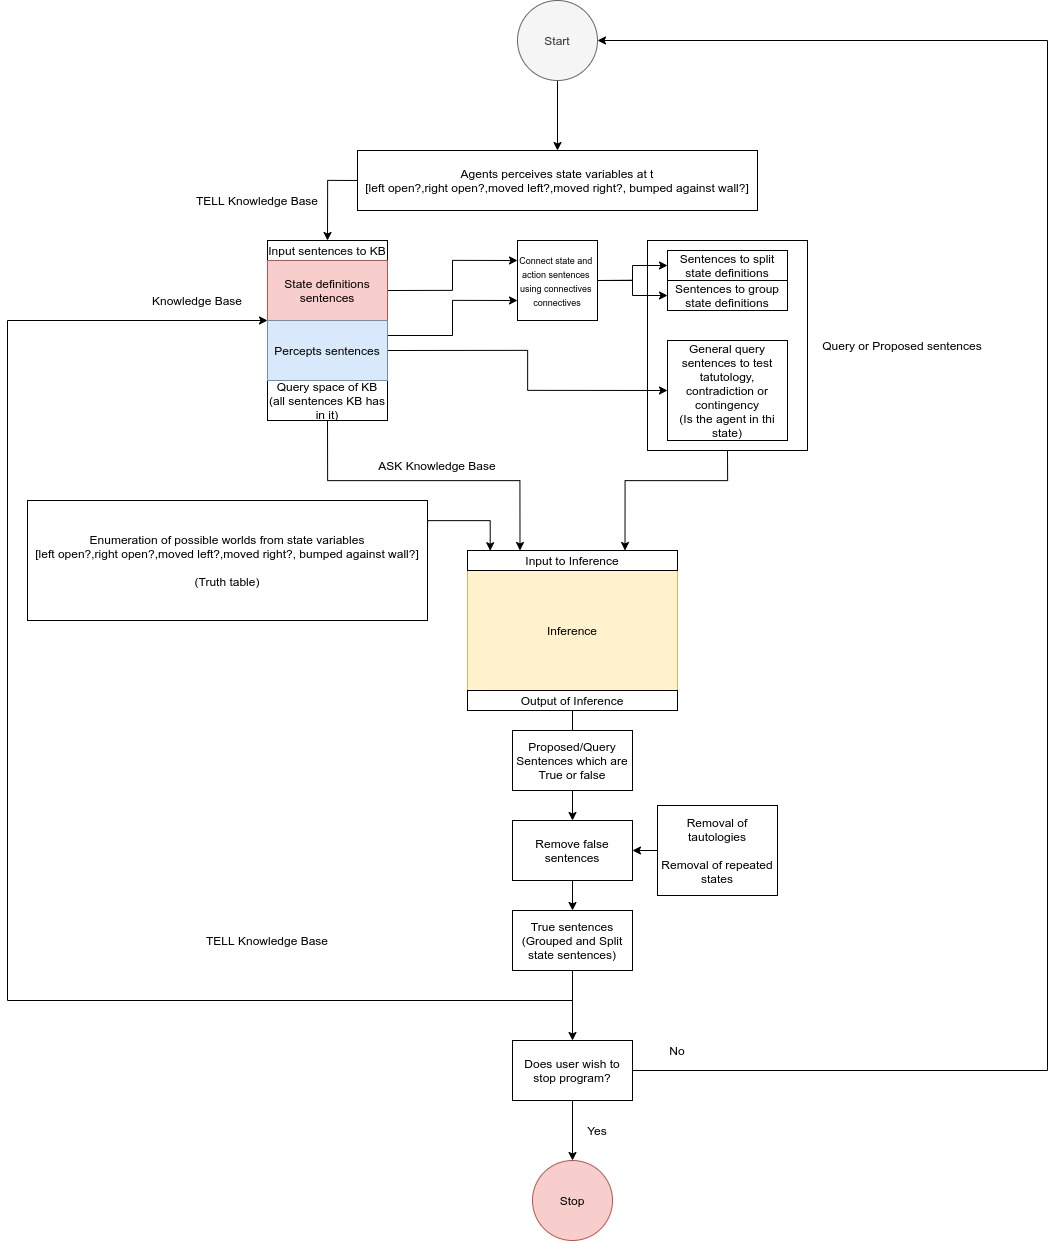
\includegraphics[scale=.3]{Figures/new_program_flow.jpg}
    \caption{Program Flow for full system} 
    \label{fig:program_flow}
\end{figure}

\section{Knowledge Base Agent}

The agent only receives percepts as inputs and action as outputs to map a representation of the environment. Thus, a percept vector (equation \ref{eq:percept_vector}) and action vector (equation \ref{eq:action_vector}) was defined. We also define a state vector (equation \ref{eq:state_vector}) using these vectors.


\begin{subequations}
\begin{align}
    \mathbf{P_t}=
\begin{bmatrix}
L_t & R_t & U_t & UL_t & UR_t & B_t & BL_t & BR_t
\end{bmatrix} 
 \label{eq:percept_vector}\\
\mathbf{A_t}=
\begin{bmatrix}
ML_t & MR_t & MU_t & MD_t & MB_t 
\end{bmatrix} 
 \label{eq:action_vector}\\
       \mathbf{S_t}=
\begin{bmatrix}
P_t & A_t  
\end{bmatrix}
 \label{eq:state_vector}
\end{align}
\end{subequations}


\section{Detailed Sub-Systems Descriptions}
\subsection{Environment}
\subsection{Knowledge Base}
\subsection{Inference Procedure}
\section{Learning Algorithms} 
\section{Forming Groups of States}
\subsection{Split State Definitions Using AND}
\subsection{Merge State Definitions Using OR}
%\citep{Discrete_Maths}
\newpage

\chapter{Testing} 



%%%%%%%%%%%%%%%%%%%%%%%%%%%%%%%%%%%%%%%%%%%%%%%%%%%%%%%%%%%%%%%%%%%%%%%%%%%%%%%%%%%%%%%
% ELO 4,6
% Planning for Conclusion

% Chapter 6: Conclusion
% This is what we tried to do...
% This is what we gave in the whole report...
% List the objectives and say which metric you uwsed and say you got the following results...

% 6.1 Objective and Results Comparison

% Objective 1...

% Objective 2...


% 6.2 So what? (Mirros Chapter 1's problem statement)
% Includes work that you found out needs to be done.
% Future work 
% Recommendations
%%%%%%%%%%%%%%%%%%%%%%%%%%%%%%%%%%%%%%%%%%%%%%%%%%%%%%%%%%%%%%%%%%%%%%%%%%%%%%%%%%%%%%

\chapter{Conclusion} 
Shows it is possible. Just one step to make the framework viable.

\label{Conclusion}
% Expert systems
\section{Results and Objectives Comparison}
\section{Improvements and Project Extensions}

\begin{itemize}
	\item Multiple Agents for Faster Learning
	\item Map Learning Agent for 3-Dimensional Environments
	\item Karnaugh Map Solver for Minimum Logic Hardware
	\item Improving the Inference Engine with First-Order Logic
	\item Implementing predictions using Hopfield Networks
\end{itemize}



%Sense input via inference
%Get true propositions
%Build State Definitions from true propositions
%Build Environment from State Definitions 
%While Environment is being build, expand State Definitions by to adding vertex descriptions
%Represent Environment in KB with expanded state definitions
%Ask via inference which state the agent is in from expanded state definitions 






\newpage

About your question: It is absolutely possible to pass your skripsie if you have not successfully solved the whole problem.  My recommendation is:

\begin{itemize}
	\item Make sure that there is a certain core part of the skripsie that you have solved, implemented and evaluated thoroughly.  It seems that you have solved the inference part?  I'd then recommend that you show that you can identify the agent state with hand-designed state definitions.  If you can compare and evaluate the 3 different inference algorithms against each other, and demonstrate that inference works for different environments, it would be good.  
	\item For the part that you would not have completed (learning the states), it is important to show how far you got.  Make sure you describe your design of the solution, which aspects of it work and for which scenarios it works (if you can show that it works for a small environment, it would be great), as well as which aspects do not yet work.  If you can explain why the parts that do not work do not work, it would be good.
	\item Do not spend too much time on trying to solve the whole problem and then not hand in a well-written report or miss the hand-in deadline.  
	\item Review the ECSA outcomes, and make sure you address all of them in your project.  
\end{itemize}

You have put a lot of effort into your project and you do have a difficult skripsie; if you can show that you have successfully solved a part of this difficult project, you should have no problem to pass (disclaimer: it will be enough for me, but I cannot predict what the internal and external examiners will think).

I suggest you continue to work hard on your project, do not throw in the towel, and make sure you hand in a well-written report.  























\chapter{Conclusion} 

\appendix%===========================================================


\backmatter%=========================================================

\bibliography{References}
\renewcommand{\thesection}{A.\arabic{section}}
\renewcommand{\thechapter}{A.}
\begin{appendix}

\setcounter{table}{0}
\renewcommand{\thetable}{A.\arabic{table}}

\chapter{Appendix A:  Project Planning Schedule}

 \begin{table}[H]
  \begin{center}
    \begin{tabular}{|c|c|p{8cm}|} 
    \hline
      \textbf{Week/Due Date} & \textbf{Starting Date} & \textbf{Description}\\
      \hline
      \hline
      1 & 06/07/2020 & Do literature study on the current map learning methods.\\ \hline
      
      2 & 13/07/2020 & Do literature study on propositional logic, 
      inference and knowledge base implementations.\\ \hline
      
      3 & 20/07/2020 & Do literature study on possible software architectures.\\ \hline
      
      4 & 27/07/2020 &  Research agent-environment interface design. \\ \hline
      
      5  & 03/08/2020 & Design agent-environment interface design.  \\ \hline
      
      6 & 10/08/2020 & Implement agent-environment interface\\ \hline
      
      7 & 17/08/2020 & Implement inference for three-states case using possible worlds. \\ \hline
      
      8 & 24/08/2020 & Finish three-states case completely.\\ \hline
      
      9 & 31/08/2020 & Expand to ambiguous-states case for one dimension.\\ \hline
      
      10 & 07/09/2020 & Expand to two-dimensional case without obstructions.\\ \hline
      
      11 & 14/09/2020 & Expand to two-dimensional case with obstructions.\\ \hline
      
      12 & 21/09/2020 & Large scale informal testing.\\ \hline
      
      13 & 28/09/2020 & Have a working model for experiments.\\ \hline
      
      14 & 05/10/2020 & Experiments, results and analysis.\\ \hline
      
      
      15 & 12/10/2020 & Supervisor checks report.\\ \hline
      
      16 & 19/10/2020 & Incorporate supervisor feedback.\\ \hline
      
      17 & 26/10/2020 & Incorporate supervisor feedback.\\ \hline
      
      Final Deadline & 09/11/2020 &  Report Hand-in 9 November\\ 
      
      \hline
    \end{tabular}
  \end{center}
  \caption{Breakdown of planning schedule per week}
    \label{tab:tablea1}
\end{table}
\setcounter{table}{0}
\renewcommand{\thetable}{B.\arabic{table}}

\vspace{-5cm}

%At the back of the report, descriptions must be provided on how these are achieved. These descriptions must be kept short, but must be actual motivations relating to the details of the work done and not only references to sections/chapters of the report.


\chapter{Appendix B: Outcomes Compliance}

\vspace{-1cm}

    
 \begin{table}[H]
  \begin{center}
    \begin{tabular}{ | p{8cm} | l | p{6cm} |}
    \hline
    
    Outcome & Chapters & Description \\ \hline \hline
    
    ELO 1. Problem solving: Identify, formulate, analyse and solve complex	engineering problems creatively and innovatively. & 1,2,3 and 4 & The problem was identified. Logic techniques were formulated. The agent design was analysed. The problem was solved. \\ \hline
    
    
    ELO 2. Application of scientific and engineering knowledge: Apply knowledge of mathematics, natural sciences,
engineering fundamentals and an engineering speciality to solve complex engineering problems. & 3 and 4 & In-depth agent design required mathematical and computer science knowledge to be applied. \\ \hline
    
    
    ELO 3. Engineering Design: Perform creative, procedural and non‐procedural design and synthesis of components, systems, engineering works, products or processes. & 3 and 4 & Agent design and implementation required creative, procedural and non‐procedural design and thinking to be applied. \\ \hline



    ELO 4. Investigations, experiments and data analysis: Demonstrate competence to design and conduct investigations and experiments & 4 and 5 & Results are given in text, figures and tables with labels and the discussions interprets results.  \\  \hline


    ELO 5. Engineering methods, skills and tools, including Information Technology: Demonstrate competence to use appropriate engineering methods, skills and tools, including those based on information technology. & 3 and 4 & Designed agent using Python and simulated experiments using Python. Finding suitable coding libraries for agent and environment implementation. \\  \hline



	ELO 6. Professional and technical communication: Demonstrate competence to communicate effectively, both orally and in writing, with engineering audiences and the community at large. & All Chapters &  Used appropriate report style and structure. Analysis of data was explained. Notation for logic explained.  \\  \hline




    ELO 8. Individual work: Demonstrate competence to work effectively as an individual & All Chapters & Learned skills to solve problem alone. All sources used were cited from. \\  \hline



    ELO 9. Independent Learning Ability: Demonstrate competence to engage in independent learning through well‐developed learning skills. & All Chapters &  Literature study explains and sources various mathematical logic methods and computer science related concepts. Developed a original agent based on logic.\\  \hline

    \hline
    \end{tabular}
\end{center}
  \caption{ Description of outcomes compliance based on relevant chapters}
    \label{tab:tableb1}
\end{table}
% \chapter{Appendix C: Environment}


\end{appendix}
\end{document}